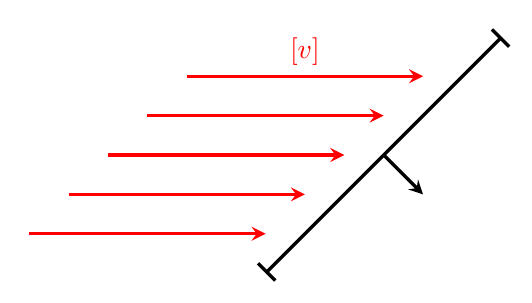
\begin{tikzpicture}[line width = 1.2pt, line join=round,x=1cm,y=1cm,>=stealth]
	% Fläche
	\draw [|-|] (0,-0.5) -- (3,2.5);
	\draw (2.8,2.5) node[anchor=east] {$\SpezialFlaeche$};
	\draw[->] (1.5,1) -- (2,0.5) node[anchor=north west] {$\normalenvektor$};
	% elektrische Stromdichte
	\foreach \s in {0,0.5,1,1.5,2} \draw[->,color=red] ({-3+\s},{\s}) -- ({\s},{\s});
	\draw [color=red] (0.5,2) node[anchor=south] {$\StromDichte[v]$};
\end{tikzpicture}